% Consulting page — working draft for gabriel.cr/consulting/
%
% THIS IS A DRAFTING FILE, NOT THE PUBLISHED SOURCE.
% The live page is ../_pages/consulting.md. Edit the prose here; when it reads
% right, tell Main to port it back into the markdown. The underscore on _src/
% means Jekyll ignores this directory, so nothing here is ever published.
%
% Structure mirrors the page 1:1 so the port back is mechanical:
%   \section{...} here  ==  "## ..." in the markdown
% Anything marked STRUCTURAL below is page furniture (HTML), not prose --
% it is shown so the flow is legible, but it is not edited as text.
%
% Content structure follows ~/MaMi/outputs/slides/mami_intro.tex (the deck).
%
% Compile:  xelatex consulting.tex

% !TEX program = xelatex
\documentclass[12pt,letterpaper]{article}

\usepackage{iftex}
\ifPDFTeX
  \usepackage[utf8]{inputenc}
  \usepackage[T1]{fontenc}
  \usepackage{ebgaramond}
\else
  \usepackage{fontspec}
  % TeX Live's EB Garamond, not the system one: that bold is a 58 kB stub with
  % no accented letters, apostrophe or dashes, and every bold accent prints as
  % a tofu box.
  \setmainfont{EBGaramond-Regular.otf}[
    Path            = /usr/share/texlive/texmf-dist/fonts/opentype/public/ebgaramond/,
    BoldFont        = EBGaramond-Bold.otf,
    ItalicFont      = EBGaramond-Italic.otf,
    BoldItalicFont  = EBGaramond-BoldItalic.otf,
  ]
\fi

% Wide right margin, for marking the draft up by hand.
\usepackage[letterpaper,left=1.1in,right=2.2in,top=1in,bottom=1in,
            marginparwidth=1.6in,marginparsep=0.25in]{geometry}
\usepackage{setspace}
\usepackage{graphicx}
\usepackage{titlesec}
\usepackage{xcolor}
\usepackage[hidelinks]{hyperref}

\definecolor{accent}{HTML}{B5735A}   % the site's terracotta
\definecolor{muted}{HTML}{6E6862}

\onehalfspacing
\setlength{\parindent}{0pt}
\setlength{\parskip}{0.7em}
\pagestyle{plain}

% Section headings echo the site: small caps, letterspaced, no numbering.
\titleformat{\section}{\normalfont\large\scshape\color{accent}}{}{0pt}{}
\titlespacing*{\section}{0pt}{1.6em}{0.5em}

% The opening question: the .lede block on the page.
\newcommand{\lede}[1]{%
  \vspace{0.3em}%
  {\color{accent}\rule{2pt}{1.5em}}\hspace{0.7em}%
  \parbox[t]{0.86\linewidth}{\vspace{-1.35em}\large\itshape #1}\par
  \vspace{0.9em}%
}

% Page furniture that is not prose.
\newcommand{\structural}[1]{{\color{muted}\small\itshape [STRUCTURAL] #1}\par}

\begin{document}

{\LARGE\scshape Consulting}\hfill{\color{muted}\small gabriel.cr/consulting/}
\vspace{0.3em}
{\color{accent}\hrule height 0.6pt}
\vspace{1.2em}

\lede{``I want to open a retail business. Where should I put it?''}

The usual answer to that question is a broker's intuition or an observation that a
particular corner has a lot of foot traffic. What an owner would rather have is 
every possible location considered, ending in a handful 
of addresses worth visiting.

\textbf{MaMi} is the tool I built to do that.

\section{An idea borrowed from biology}

How do biologists map where a jaguar could live, without following jaguars
around the whole country? They take the places where jaguars \emph{are}, ask what
those places have in common (forest cover, water, prey, elevation, distance
from roads), and then find every other place that looks like that. They learn
the jaguar's \textbf{habitat}.
Ecologists call these species distribution models, and they are standard practice 
in conservation planning and in predicting where an invasive species will spread next.

A business also has a habitat. Take, for example, pharmacies in Guadalajara, Mexico.

Mexico's business census records every establishment in the country twice a
year, which gives roughly a dozen photographs of the city's commerce between
2016 and 2026. Following each pharmacy across that decade lets MaMi learn the
pharmacy's environment: which socioeconomic variables determine where a pharmacy
flourishes?

\section{How the model sees the city}

A city is cut into hexagons, each about 165 meters across. For
each hexagon we ask: what is the surrounding area like? What is the habitat there?

For each hexagon's surrounding area, the model looks at three things: \textbf{who
lives there} (population, ages, schooling, household size, income proxies, how
fast the area has grown since 2010), \textbf{what is already there} (every other
business by type, hospitals, schools, offices, how mixed the street life is),
and \textbf{how reachable it is} (street layout, main avenues, bus and metro stops,
parks and markets). That comes to more than 400 signals per hexagon. The model finds the habitat
by comparing places where pharmacies flourished against places where none did.

One map answers three different business questions --- 
where there is an open opportunity with no pharmacy nearby,
where there is room for one more, and where the pharmacy deserts are.

\begin{figure}[h]
  \centering
  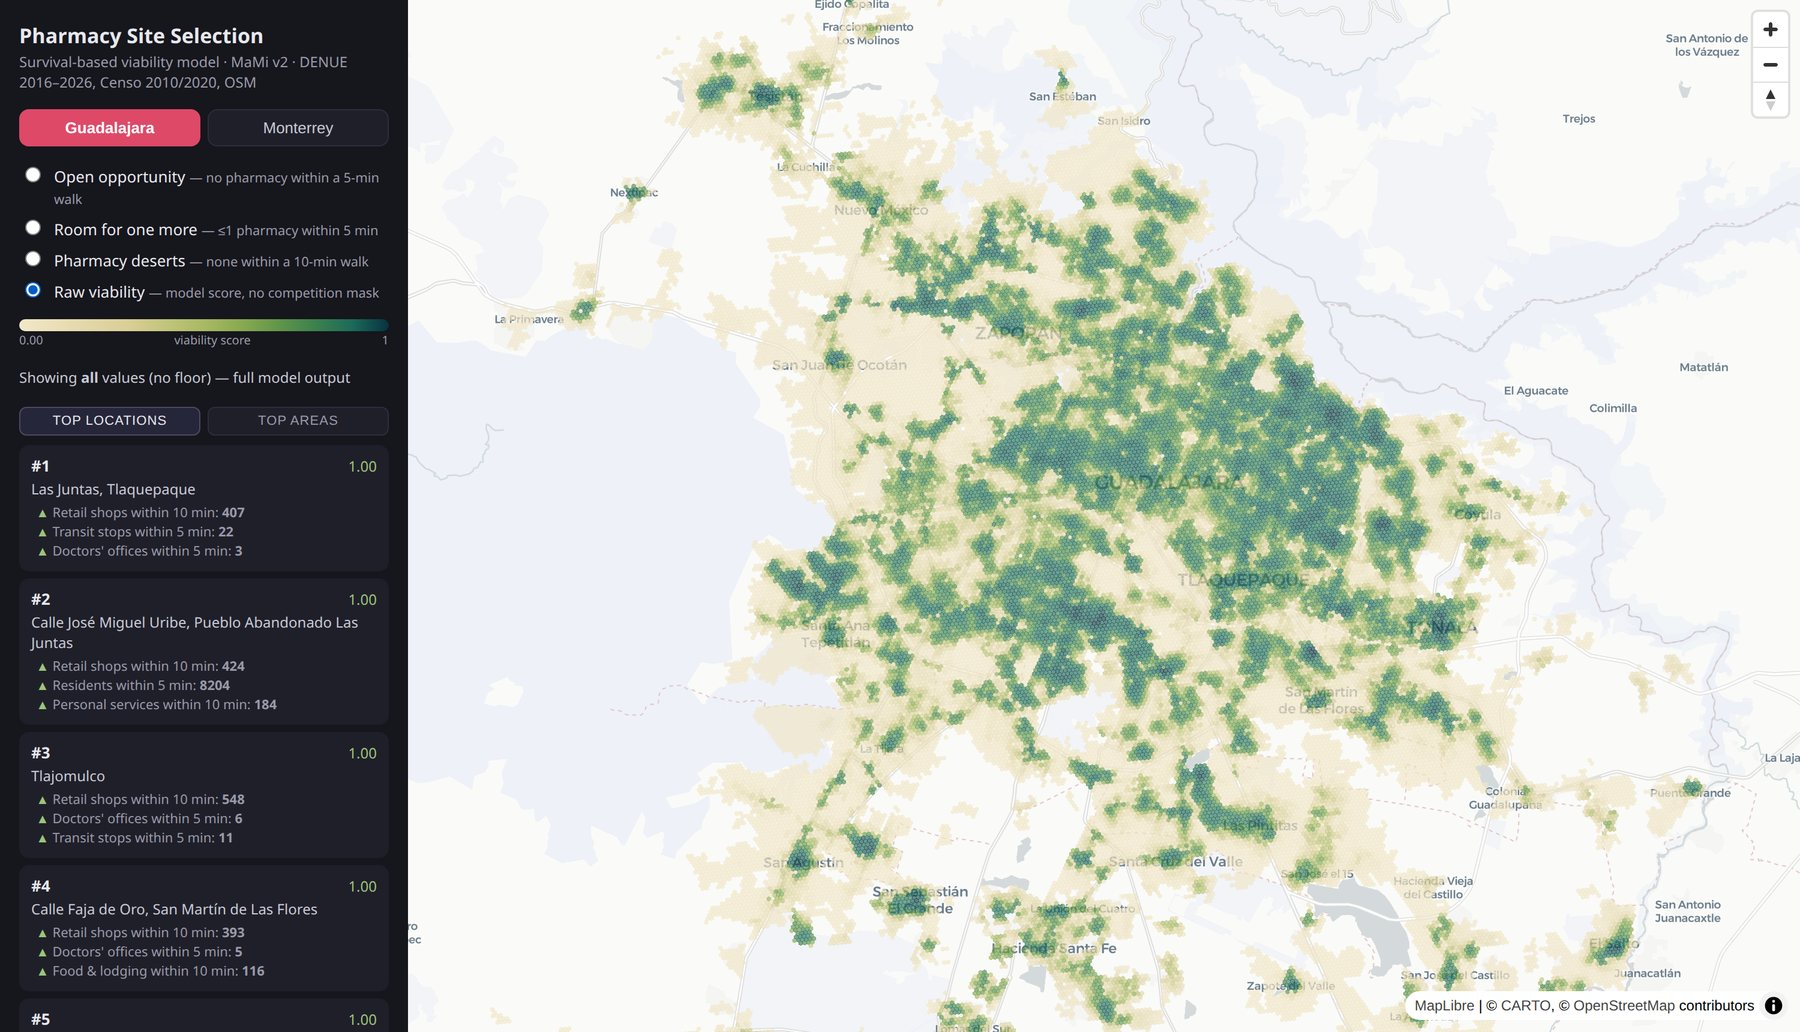
\includegraphics[width=\linewidth]{../assets/images/mami_habitat_gdl.jpg}
  \vspace{0.3em}
  {\footnotesize\color{muted}\itshape
   The result: a habitat suitability map for pharmacies in Guadalajara.\par}
\end{figure}

\section{In practice}

I built MaMi at \textbf{R2}, a market research firm in Guadalajara, and worked with it
there from 2020 to 2024. Eight successful businesses opened on its recommendations, including
pharmacies, clinical laboratories and restaurants.

What a client receives is a score for every location in the metro area; a ranked
shortlist of addresses, or of zones, when a whole area is promising; the reasons
behind each score; and an interactive map they can explore.
Change the business type (a café, a gym, a clinic), and the same machinery
re-learns that habitat from scratch.

\section{See it}

\structural{Callout card linking to /mami/. Title, then the two lines below.}

\textbf{MaMi --- Pharmacy site selection $\rightarrow$}

The pharmacy habitat map for Guadalajara and Monterrey.
{\footnotesize\color{muted}\itshape
This is a sample. It uses only a subset of the model's variables. It is meant to
show the method, not to site a business.\par}

\end{document}
